\newpage
\section{Extending the Leitner's Box GUI}
\genHeader

\vspace{0.5cm}

In addition to \texttt{removeCard}, the GUI is able to access and operate the \texttt{check} method using your SDM implementation! To avoid errors however, its
currently commented out, so you'll need to release it. First, double check and make sure your metamodel is built, and that you have correctly imported the GUI.

\begin{itemize}

\item[$\blacktriangleright$] Go to ``Other Projects/LeitnersBox/Src'' and open \texttt{LeitnersBoxController.java} in the package.

\vspace{0.5cm}

\item[$\blacktriangleright$] Beside the scrollbar on the right side of the text editor, you should be able to see two blue rectangles. Click the second one
to skip ahead to the commented line (Fig.~\ref{fig:remComment}).

\vspace{0.5cm}

\begin{figure}[htp]
\begin{center}
  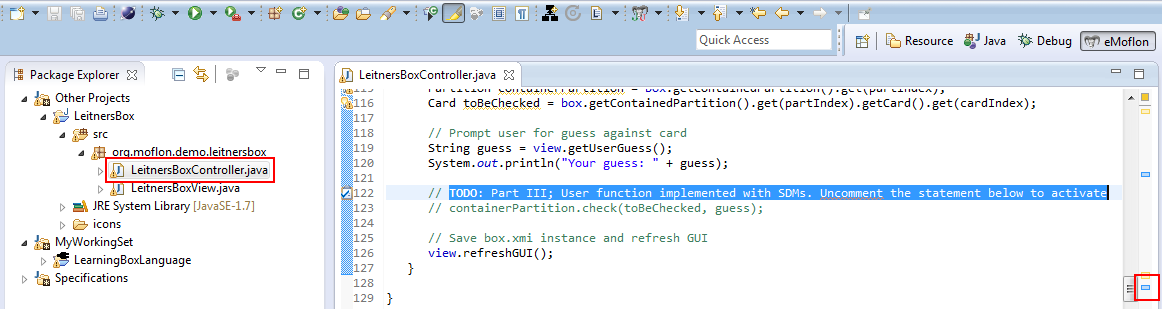
\includegraphics[width=\textwidth]{eclipse_GUICommentLine}
  \caption{Remove the comment operator on line 123}
  \label{fig:remComment}
\end{center}
\end{figure}

\vspace{0.5cm}

\item[$\blacktriangleright$] Activate the line below the highlight, save the file, then take your GUI for a spin! Experiment with
making right and wrong guesses, and watch how your cards move through the box. Try editing your instance file by making more partitions, cards and
new \texttt{FastCard}s, to see how they all interact with one another.

\end{itemize}
